\section{Overview}
\begin{itemize}
    \item Are similar to the concept of indirection.
    \item Running errands is a concept of indirection, when you ask someone to do something, and they do it that's indirection. 
    \item In programming languages, indirection is the ability to reference something using a name, reference, or container, instead of the value itself. 
    \item The most common form of indirection is the act of manipulating a value through its memory address.
    \item A pointer provides an indirect means of accessing the value of a particular data item:
        \begin{itemize}
            \item A variable whose value is a memory address.
            \item Its value is the address of another location in memory that can contain value. 
        \end{itemize}
    
    \item It makes sense to use pointers in the same respect to the initial example of the utility of addresses, C pointers are one of the most powerful tools, pointers are the most complicated concept in C. 
    \item The compiler must know the type of data stored in the variable to which it points: 
        \begin{itemize}
            \item Needs to how much memory is occupied or how to handle the contents of memory to which it points. 
            \item Every pointer will be associated with a specific variable type. 
            \item It can be used only to point to variables of that type.  
        \end{itemize}
    
    \item Pointers of type pointer int can only point to type int variables. 
\end{itemize}

\begin{figure}[H]
    \centering
    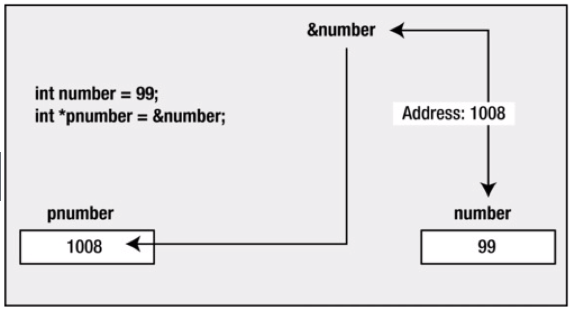
\includegraphics[width=14cm]{\figs/pointers} 
    \caption{Taken from beginning C, Horton.}
\end{figure}

\begin{itemize}
    \item A pointer has a value to an address, the value of \&number is the address where number is located. This value is used to initialize pnumber in the second statement. 
    \item What a pointer holds is the value of an address to a variable. 
\end{itemize}
\subsection{Why use pointers?}
\begin{itemize}
    \item Accessing data by means of only variables is very limiting.
        \begin{itemize}
            \item With pointers, you can access any location, you can treat any position of memory as a variable for example, and in addition perform arithmetic with pointers.
        \end{itemize}
    
    \item Pointers in C make it easier to use arrays and strings.
    \item Pointers allow you to refer to the same space in memory from multiple locations:
        \begin{itemize}
            \item This means that you can update memory in one location and the change can be seen from another location in you program. 
            \item Can also save space by being able to share components in you data structures. 
        \end{itemize}
    
    \item Pointers allow functions to modify data passed to them as variables: 
        \begin{itemize}
            \item Pass by reference: by arguments to function in way they can be changed by function. 
        \end{itemize}
    
    \item Can also be used to optimize a program to run faster or use less memory than it would otherwise use. 
    \item Pointers allow us to get multiple values from the function.
        \begin{itemize}
            \item A function can only return one value, but by passing arguments as pointers we can get more than one values from the pointer. 
        \end{itemize}
    
    \item With pointers dynamic memory can be created according to the program use:
        \begin{itemize}
            \item We can save memory from static (compile time) declarations.
        \end{itemize}
    
    \item Pointers allow us to design and develop complex data structures like stack, queue, or linked lists.
    \item Pointers provide direct memory access.
    \item Allows encapsulating global variable in functions as well.
\end{itemize}


%----------------------------------------------------------------------------------------
\section{Defining pointers}
\begin{itemize}
    \item A pointer is not declared the same way as a normal variable, you can't say: \verb|pointer ptr;|.
    \item It is not enough to say that a variable is a pointer: 
        \begin{itemize}
            \item You can also have to specify the kind of variable to which the pointer points. 
            \item Different variable types take up different amounts of storage in memory. 
            \item Some pointer operations require knowledge of that storage size. 
        \end{itemize}
    
    \item You declare a pointer to a variable of type int with syntax: \verb|int *pnumber;|
    \item The type of the variable with the name pnumber is \verb|int*|:
        \begin{itemize}
            \item Can store the addresses of any variable of type int. 
        \end{itemize}
    \item Syntax is: \placeholder{data type} *\placeholder{variable name};
    \item Types matter.
    \item The space between the * and the pointer name is optional:
        \begin{itemize}
            \item Programmers use the space in declaration and omit it when dereferencing a variable. 
        \end{itemize}
    
    \item The value of a pointer is an address, and it is represented internally as an unsigned integer on most systems. 
        \begin{itemize}
            \item However, you shouldn't think of a pointer as an integer type. 
            \item There are things you can do with integers that you can not do with pointers, and vice versa.
            \item You can multiply one integer by another, but you can not multiply one pointer by another. 
        \end{itemize}
    
    \item A pointer is really a new type, not an integer type. 
        \begin{itemize}
            \item \%p represents the format specifier for pointers.
        \end{itemize}
    
    \item The previous declarations create the variable but do not initialize it: 
        \begin{itemize}
            \item Dangerous when not initialized. 
            \item You should always initialize a pointer when you declare it. 
        \end{itemize}
\end{itemize}
\subsection{NULL Pointers}
\begin{itemize}
    \item You can initialize a pointer so that it does not point to anything. \verb|int *pnumber = NULL;|
    \item NULL is a constant that is defined in the standard library, it is the equivalent of zero for a pointer. 
    \item NULL is a value that is guaranteed not to point to any location in memory:
        \begin{itemize}
            \item Means that it implicitly prevents the accidental overwriting of memory by using a pointer that does not point to anything specific. 
        \end{itemize}
    
    \item NULL is not \verb|\0| character in strings they are diferent. 
    \item Add an \#include directive for stddef.h to your source file. 
\end{itemize}
\subsection{Address of operator}
\begin{itemize}
    \item If you want to initialize your variable with the address of a variable you have already declared:
        \begin{itemize}
            \item Use the address of operator \verb|&|.
        \end{itemize}
            \begin{minted}[autogobble]{c}
                int number = 99;
                int *pnumber = &number; 
            \end{minted}
    
    \item The initial value of pnumber is the address of the variable number. 
        \begin{itemize}
            \item The declaration of number must precede the declaration of the pointer that stores its address.
            \item Compiler must have already allocated space and thus address for number to use it to initialize pnumber.
        \end{itemize}    
\end{itemize}

\subsection{Precautions}
\begin{itemize}
    \item There is nothing special about the declaration of a pointer: 
        \begin{itemize}
            \item You can declare regular variables and pointers in the same statement: \mintinline{c}{double value, *pVal, fnum;}
        \end{itemize}
    
    \item Only the second variable pVal is a pointer.
    \item \verb|int *p,q;| this declaration is of a pointer of type int* and a variable q of type int; a common mistake is to think that both p and q are pointers.
    \item Also, a good idea to use names beginning with p as pointer names. 
\end{itemize}

%----------------------------------------------------------------------------------------
\section{Accessing pointers}
\subsection{Access pointer values}
\begin{itemize}
    \item You can use the indirection operator *, to access the value of the variable pointed to by a pointer; also referred to as the deference operator because you use it to ``dereference'' a pointer.
        \begin{minted}[autogobble]{c}
            int number = 15; // to get this value
            int *pnumber = &number;
            int result = 0; 
        \end{minted}
    
    \item To get this value: the pointer variable contains the address of the variable number:
        \begin{itemize}
            \item You can use this in an expression to calculate a new value for result.
        \end{itemize}
    \begin{minted}[autogobble]{c}
        result = *pointer + 5; // result is 20 
    \end{minted}
    
    \item The expression *pointer will evaluate to the value stored at the address contained in the pointer:
        \begin{itemize}
            \item The value stored in number, 15, so result will be set to 15 + 5, which is 20.
        \end{itemize}
    
    \item The indirection operator, *, is also the symbol for multiplication, and it is used to specify pointer types:
        \begin{itemize}
            \item Depending on where the asterisk appears, the compiler will understand whether its should interpret it as an indirection operator, as multiplication sign, or as part of a type specification.
            \item Context determines what it means in any instance. 
        \end{itemize}
    
    \item Dereferencing is the process of which through a pointer I'm able to obtain the value stored in the variable of which the pointer is pointing to. 
    \inputcode{\lang}{\code/dereferencing.c}
\end{itemize}

\subsection{Displaying a pointer's value}
\begin{itemize}
    \item To output the address of a variable, you use the output format specifier \%p:
        \begin{itemize}
            \item Outputs a pointer value as a memory address in hexadecimal form.
        \end{itemize}
    \inputcode{\lang}{\code/displaying_pointers.c}
    
    \item Pointers occupy 8 bytes (depending on you machine) and the addresses have 16 hexadecimal digits:
        \begin{itemize}
            \item If a machine has 64-bit operating system and my compiler supports 64-bit addresses, some compilers only support 32-bit addressing, in which case addresses will be 32-bit addresses. 
        \end{itemize}
    
    \item Remember, a pointer itself has an address, just like any other variable:
        \begin{itemize}
            \item You use \%p as the conversion specifier to display an address. 
        \end{itemize}
    
    \item You use the \& (address of) operator to reference the address that the pnumber variable occupies.
    \item The cast to void* is to prevent a possible warning from the compiler: 
        \begin{itemize}
            \item The \%p specification expects the value to be kind of pointer type, but the type of \&pnumber is ``pointer to a pointer to int''.
        \end{itemize}
\end{itemize}

\subsection{Displaying a number of bytes you are using}
\begin{itemize}
    \item You use the sizeof operator to obtain the number of bytes a pointer occupies:
        \begin{itemize}
            \item On my machine this shows that a pointer occupies 8 bytes.
            \item A memory address on my machine is 64 bits.
        \end{itemize}
    
    \item You may get a compiler warning when using sizeof this way:
        \begin{itemize}
            \item size\_t is an implementation-defined integer type. 
            \item To prevent the warning, you could cast the argument to type int like this: 
            \begin{minted}[autogobble]{c}
                printf("pnumber's size: %d bytes\n",(int)sizeof(pnumber)); 
            \end{minted}
        \end{itemize}
\end{itemize}
\inputcode{\lang}{\code/accessing_pointers.c}


%----------------------------------------------------------------------------------------
\section{Challenge}
\inputcode{\lang}{\code/pointer_basics.c}


%----------------------------------------------------------------------------------------
\section{Overview}
\begin{itemize}
    \item C offers several basic operations you can perform on pointers.
    \item You can assign an address to a pointer:
        \begin{itemize}
            \item Assigned value can be an array name, a variable preceded by address operator \&, or another second pointer. 
        \end{itemize}
    
    \item You can also dereference a pointer: 
        \begin{itemize}
            \item The * operator gives the value stored in the pointed-to location.
        \end{itemize}
    
    \item You can take a pointer address:
        \begin{itemize}
            \item The \& operator tells where the pointer itself is stored.
        \end{itemize}
    
    \item You can perform pointer arithmetic:
        \begin{itemize}
            \item Use the + operator to add an integer to a pointer or a pointer to an integer (integer is multiplied by the number of bytes in the pointed-to type and added to the original address) 
            \item Increment a pointer by one (useful in arrays when moving to the next element)
            \item Use the — operator to subtract an integer from a pointer (integer is multiplied by the number of bytes in the pointed-t type and subtracted from the original address).
            \item Decrementing a pointer by one (useful in arrays when going back to the previous element) this means when you're iterating an array and you don't want to use the index, you can increment it by one. 
        \end{itemize}
    
    \item You can find the difference between two pointers:
        \begin{itemize}
            \item You do this for two pointers to elements that are in the same array to find out how far apart the elements are. Example: you have a pointer to index 5 and a pointer to index 15 in an array you can subtract the pointers and find the difference. 
        \end{itemize}
    
    \item You can use the relational operators to compare the values of two pointers:
        \begin{itemize}
            \item Pointers must be the same type.
            \item This means you can find out if an address is greater than another. 
        \end{itemize}
    
    \item Remember, there are two forms of subtraction:
        \begin{itemize}
            \item You can subtract one pointer from another to get an \textbf{integer}.
            \item You can subtract an integer from a pointer and get a \textbf{pointer}.
        \end{itemize}
    
    \item Be careful when you use incrementing or decrementing pointers and causing an array ``out of bounds'' error:
        \begin{itemize}
            \item Computer does not keep track of whether a pointer still points to an array element or to another arbitrary point in memory. 
            \item If you increment too much in an array using pointer arithmetic you will get an array ``out of bounds'', if you decrement the array too much you will get an ``under bounds'' error, this will be apparent in debugging since these errors are that occur in runtime, not compile time. 
        \end{itemize}
    
    \item The value referenced by a pointer can be used in arithmetic expressions:
        \begin{itemize}
            \item If a variable is defined to be if type ``pointer to integer'' then it is evaluated using the rules of integer arithmetic. 
        \end{itemize}
            \begin{minted}[autogobble]{c}
                int number = 0; 
                int *pnumber = NULL; 
                number = 10; 
                pnumber = &number; 
                *pnumber += 25; // The value pointed to is incremented to 25
            \end{minted}
    \begin{itemize}
        \item Increment the value of the number variable by 25. 
    \end{itemize}
        \begin{itemize}
            \item * indicates you are accessing the contents to which the variable called pnumber is pointing to. 
        \end{itemize}
    
    \item If a pointer pointes to a variable x:
        \begin{itemize}
            \item That pointer has been defined to be a pointer to the same data type as is x. 
            \item Using the *pointer in an expression is identical to the use of x in the same expression. 
        \end{itemize}
    
    \item A pointer can contain the address of any variable of the appropriate type:
        \begin{itemize}
            \item You can use one pointer variable to change the values of many variables. 
            \item As long as they are of type compatible with the pointer type. 
        \end{itemize}
    \inputcode{\lang}{\code/using_pointers.c}
\end{itemize}

\subsection{When reciecing input}
\begin{itemize}
    \item When we have used scanf() to input values, we used the \& operator to obtain the address of a variable:
        \begin{itemize}
            \item On the variable os that is to store the input. 
            \item We used \& on all variables except the character array because the array name is a a character pointer. 
        \end{itemize}
    \item scanf()'s second argument is a pointer, so whenecer you have a pointer that already contains an address, you can use the pointer name as an argument for scanf(). 
        \begin{minted}[autogobble]{c}
            int value = 0; 
            int *pvalue = &value; 
            printf("Input an integer: ");
            scanf("%d",pvalue); 
            printf("You entered %d.\n",value); 
        \end{minted}
    
\end{itemize}

\subsection{Testing for NULL}
\begin{itemize}
    \item There is one rule you should burn into you memory.
        \begin{itemize}
            \item Do not dereferene an uninitialized pointer. 
        \end{itemize}
            \begin{minted}[autogobble]{c}
                int *pt; // uninitialized pointer. 
                *pt = 5 // terrible error. 
            \end{minted}
    
    
    \item The second line means store the value 5 in the location to hoch pt points: 
        \begin{itemize}
            \item pt has random value, there is no knowing ehre 5 will be placed. 
            \item It can be be placed anywhere in memory, this might be harmless or might overwrite data or code, or it might cause the program to crash. 
        \end{itemize}
    
    \item Creating a pointer only allocates memory to store the pointer itself:
        \begin{itemize}
            \item It does not allocate memory to store data, only to hold the pointer itself, youb can't dereference it. 
            \item Before you use a pointer, it should be assigned a memory location that has already been allocated.
                \begin{itemize}
                    \item Assign the address of an existing variable to the pointer. 
                    \item Or you can use dynamic memory allocation with the malloc() function to allocate memory first. 
                \end{itemize}
            
            \item So if you create a variable always initialize it to NULL and test your code for null pointers. 
        \end{itemize}
    
    \item You can test for NULL to make sure you don't have a dereferencer and your program doesn't crash: 
        \begin{itemize}
            \item We already know that when declaring a pointer that does not point to anything, we should initialize it to NULL. NULL points to nothing. \verb|int *pvalue = NULL; |
            \item NULL is a special symbol in C that represents the pointer equivalent to 0 with ordinary numbers.
            \item Another way to set a poiter to NULL is to assign it to zero. \verb|int *pvalue = 0;|
            \item Because NULL is the equivalent of zero, if you want to test whether pvlue is NULL, you can do this \verb|(pvalue == NULL)| OR \verb|if (!pvalue) {<code>;}|.
            \item You want to check for NULL before you dereference a pointer:
                \begin{itemize}
                    \item Often when pointers are passed to functions, functions use pointers as parameters, if the caller is passing in bad data that doesn't have memory allocated it can crash you code, this you must do always in functions, always have these checks. 
                    \item To avoid crashes. 
                \end{itemize}
        \end{itemize}
\end{itemize}


%----------------------------------------------------------------------------------------
\section{Pointes and const}
\begin{itemize}
    \item When we use the const modifier on a variable or array it tells the compiler that the contents of the variable/array will not be changed by the program.
    \item With pointers, we have to consider two things when using const modifiers:
        \begin{enumerate}
            \item Whether the pointer will be changed 
            \item Whether the value that the pointer points to will be changed.
        \end{enumerate}
\end{itemize}

\subsection{Pointers to constants}
\begin{itemize}
    \item You can use the const keyword when you declare a pointer to indicate that the value pointed to must be changed. 
    \item Syntax is: const \placeholder{type} *\placeholder{name} = \placeholder{address}; 
        \begin{minted}[autogobble]{c}
            long value = 9999L; 
            const long *pvalue = &value; // defines pointer to a cosntant. 
        \end{minted}

    \item You have declared the value pointed to by pvalue to be cosnt. 
        \begin{itemize}
            \item The compiler will check for any statements that attempt to modify the value pointed to by the pvalue and flag such statements as an error. 
        \end{itemize}
    
    \item The following statement will now result in an error message from the compiler: 
        \begin{minted}[autogobble]{c}
            *pvalue = 8888L; // Error - attempt to change const location. 
        \end{minted}
    
    
    \item We would still be able to change value, we just can't change *pvalue. Value is defined as a long not a constant so value can be changed but you can't change the pointer to a constant. You applied const to the pointer. 
        \begin{minted}[autogobble]{c}
            value = 7777L; // allowed
        \end{minted}
 
    
    \item The value pointer to has changed, but you did not use the pointer to make the change, you used the variable. 
    \item The pointer itself is not a constant, it's a pointer to constant, we declared the pointer to be of type pointer to constant, you can still change what it points to. 
        \begin{minted}[autogobble]{c}
            long number = 8888L; 
            pvalue = &number; // OK - Changing the address in pvalue.
        \end{minted}
    
    \item Will change the address stored in pvalue to point to number. 
        \begin{itemize}
            \item Still, cannot use the pointer to change the value that is stored. 
            \item You can change the address stored in the pointer as much as you like. 
            \item Using the pointer to change the value pointed to is not allowed, even after you have reached the address stored in the pointer. 
        \end{itemize}
\end{itemize}

\subsection{Constant pointers}
\begin{itemize}
    \item You might also want to ensure that the address stored in the pointer cannot be changed. 
    \item You can do this by using the const keyword in the declaration of the pointer. 
    \item Syntax is: \placeholder{type} *\placeholder{const} \placeholder{name} = \placeholder{constant address}; 

        \begin{minted}[autogobble]{c}
            int count = 43; 
            int *const pcount = &count; // defines constant pointer
        \end{minted}

    
    \item The above ensures that a pointer always points to the same thing. 
        \begin{itemize}
            \item It indicates that the address stored must not be changed. 
            \item Compiler will check that you do not inadvertently attempt to change what the pointer points to elsewhere in your code.  
        \end{itemize}
            \begin{minted}[autogobble]{c}
                int item = 34; 
                pcount = &item; // Error - attempt to change a constant pointer. 
            \end{minted}
    
    
    \item Its all about where you place the const keyword, either before the type or after the type. 
        \begin{minted}[autogobble]{c}
            const int * // value can not be changed. 
            int *const // pointer address cannot change 
        \end{minted}
    
    \item You can still change the value that pcount points to using pcount.
        \mint{c}{*pcount = 345; // Ok - changes the value of count}
    \item References the value stored in count through the pointer and changes its value to 345. 
    \item You can create a constant that points to a value that is also a constant: 
        \begin{minted}[autogobble]{c}
            int item = 25; 
            const int * const pitem = &item;
        \end{minted}
    \item The pitem is a constant pointer to a constant so everything is fixed, you cannot:
        \begin{enumerate}
            \item Change the address stored in pitem. 
            \item Use pitem to modify what it points to. 
        \end{enumerate} 
    
    \item You can still change the value of item directly:
        \begin{itemize}
            \item If you wanted to make everything not change, you could specify item as const as well. That will make it so that the pointer and the variable cannot change. 
        \end{itemize}
\end{itemize}

%----------------------------------------------------------------------------------------
\section{Void pointers}
\begin{itemize}
    \item Remember a void function, a void function was a function that did not return anything. 
    \item The type name void means absence of any type. 
    \item A pointer of type void* can contain the address of a data item on \textbf{any} type. This allows for a lot of flexibility. 
    \item void* is often used as a parameter type or return value type with functions that deal with data in type-independent way. 
    \item Any kind of pointer can be passed around as a value of type void* : 
        \begin{itemize}
            \item The void pointer does not know what type of object it is pointing to, so, it cannot be dereference directly (this is the part that isn't flexible, you can only use it if you know what to cast it).
            \item The void pointer must first be explicitly cast to another pointer type before it is dereferenced. 
        \end{itemize}
    
    \item The address of a variable of type int can be stored in a pointer variable of type void*. 
    \item When you want to access the integer value at the address stored in the void* pointer, you must first cast the pointer to type int*.
    \item To dereference it the syntax is: (\placeholder{data type} *)\placeholder{void *pointer}
\end{itemize}
\inputcode{\lang}{\code/void_pointers.c}

%----------------------------------------------------------------------------------------
\section{Pointers and arrays}
\begin{itemize}
    \item There is a strong relationship between pointers and arrays. 
    \item An array is a collection of objects of the same type that you can refer to using a single name. 
    
    \item A pointer is a variable that has as its value a memory address that can reference another variable or constant of a given type: 
        \begin{itemize}
            \item You can use a pointer to hold the address of different variables at different times (must be same type).
            \item You must have the same type. 
        \end{itemize}
    
    \item Arrays and pointers seem quite different, but, they are very closely related and can sometimes be used interchangeably. 
    \item One of the most common uses of pointers in C is as pointers to arrays. 
    \item The main reason for using pointers to arrays are ones of notational convenience and of program efficiency. 
    \item Pointers to arrays generally results in code that uses less memory and executes faster. 
    \item Use pointers over arrays. 
    \item If you have an array of 100 integers:
        \begin{minted}[autogobble]{c}
            int values [100];
        \end{minted}
    
    \item You can define a pointer called valuesPtr, which can be used to access the integers contained in this array: 
        \begin{minted}[autogobble]{c}
            int *valuesPtr;
        \end{minted}
    
    \item When you define a pointer that is used to point to the elements of an array, you do not designate the pointer as type ``pointer to array''
        \begin{itemize}
            \item You designate the pointer as pointing to the type of element that is contained in the array. 
        \end{itemize}
    
    \item To set the valuesPtr to point to the first element in the values array, you write: 
        \begin{minted}[autogobble]{c}
            valuesPtr = values; // this is going to point to the first address in the array
        \end{minted}
        \begin{itemize}
            \item Note we don't use the \& operator, this is because arrays are themselves pointers. 
        \end{itemize}
    
    \item The address operator is not used: 
        \begin{itemize}
            \item The C compiler treats the appearance of an array name without a subscript as a pointer to the array. 
            \item Specifying values without a subscript has the effect of producing a pointer to the first element of values.
        \end{itemize}
\end{itemize}

\subsection{Arrays and pointers}
\begin{itemize}
    \item An equivalent way of producing a pointer to the start of values is to apply the address operator to the first element of the array. You can use this one:  
        \begin{minted}[autogobble]{c}
            valuesPtr = &values[0]; // this is maybe clearer, since you don't know that values is an array. 
        \end{minted}
        or 
        \begin{minted}[autogobble]{c}
            valuesPtr = values; // shortcut, unclearer.
        \end{minted}
    
    \item Either one is fine and matter of programmer preference. 
\end{itemize}

\subsection{Summary}
\begin{itemize}
    \item The two expressions \mintinline{c}{ar[i]} and \mintinline{c}{*(ar+i)} are equivalent in meaning.
        \begin{itemize}
            \item Both work if \mintinline{c}{ar} is the name of an array, and both work if \mintinline{c}{ar} is a pointer variable. 
            \item Using an expression such as \mintinline{c}{ar++} only works if \mintinline{c}{ar} is a pointer variable. 
        \end{itemize}
\end{itemize}

%----------------------------------------------------------------------------------------
\section{Pointer Arithmetic}
\begin{itemize}
    \item Don't be mislead by the name ``arithmetic'', itself just means adding or subtracting to a pointer.
    \item The real power of using pointers to arrays comes into play when you want to sequence through the elements of an array.
    \item Because each element of an array is an address, you can iterate through them using pointer arithmetic. 
    \mint{c}{*valuesPtr // can be used to access the first intever to the values array, that is, values[0]}
    \item To reference values[3] through the valuesPtr variable, you can add 3 to valuesPtr and then apply the indirection operator. 
    \mint{c}{*(valuesPtr + 3)}
    
    \item This is going to multiply the bites times the integers. This is essentially going to point to the third element in the array. 
    \item The expression, \mintinline{c}{*(valuesPtr+i)} can be used to access the value contained in values[i].
        \begin{itemize}
            \item To set values[10] to 27, you coud fo the following. 
        \end{itemize}
        \begin{minted}[autogobble]{c}
            values[10] = 27; 
            // or, using valuesPtr, you could
            *(valuesPtr + 10) = 27;
        \end{minted}
    
    \item Pointer arithmetic is notationally rigorous, however, it allows for a faster and more memory efficient way to access and modify array elements. 
    \item To set valuesPtr to point to the seccond element of the values array, you can apply the address of operator to values[1] and assign the result o valuesPtr. 
    \mint{c}{valuesPtr = &values[1];}
    
    \item it valuesPtr points to values[0], you can set it to point to values[1]by simply adding 1 to the values of valuesPtr. 
    \mint{c}{valuesPtr += 1;}
    
    \item This is a perfectly valid expression in C can be used for pointers to any data type. 
    \item The increment and decrement operators ++ and -- are particularly useful when dealing with pointers. 
        \begin{itemize}
            \item Using the increment operator on a pointer has the same effect as adding one to the pointer. 
            \item Using the decrement operator has the same effect as subtracting one from the pointer. 
        \end{itemize}
    \mint{c}{++valuesPtr;}
    \item Sets valuesPtr pointing to the next integer in the values array (values[1]).
    \mint{c}{--valuesPtr;}
    \item Sets valuesPtr pointing to the previous integer in the values array, assuming that valuesPtr was not pointing to the beginning of the values array. 
    \item Be careful with: Out of bounds errors.
\end{itemize}

\subsection{Example}
\inputcode{\lang}{\code/pointer_arithmetic.c}
\begin{itemize}
    \item To pass an array to a function, you simply specify the name of the array. 
    \item To produce a pointer to an array, you need only to specify the name of the array.
    \item This implies that in the call to the arraySum() function, what was passed to the function was actually a pointer to the array values:
        \begin{itemize}
            \item This explains why you are able to change the elements of an array from within a function considering a function can only change variables inside the function scope. 
            \item An array is nothing more than a pointer.
            \item This is why we pass in the elements for the scanf() function. 
        \end{itemize}
    
    \item SO, why the formal parameter inside the function is not declared to be a pointer?
        \mint{c}{int arraySum(int *array, const in n);}
        \begin{itemize}
            \item The above is perfectly valid. 
            \item Pointers and arrays are intimately related in C. 
            \item This is why you can declare arrays to be of type ``array of ints'' inside the arraySum function or to be of type ``pointer to int''.
            \item This is why you see many functions accept arrays as parameters, the array is in itself a pointer. 
        \end{itemize}
    
    \item If you are going to be using index numbers to reference the elements of an array that is passed to a function, declare the corresponding formal parameter to be an array. 
        \begin{itemize}
            \item More correctly reflects the use of the array by the function. 
        \end{itemize}
    
    \item In terms of notation, for simplicity and less code and clarity (if you understand pointers) you might want to use pointers instead of indexes. 
\end{itemize}

\subsection{Summary}
\begin{minted}[autogobble]{c}
    int urn[3]; 
    int *ptr1, *ptr2;
\end{minted}
\begin{center}
    \begin{tabular}{ |p{7cm}|p{7cm}| }
        \hline
            Valid & Invalid \\
        \hline
            ptr1++;  & urn++; \\ 
            ptr2 = ptr1 + 2; & ptr2 = ptr2 + ptr1; \\ 
            ptr2 = urn + 1 & ptr2 = urn *ptr1; \\ 
        \hline
    \end{tabular}
\end{center}
\begin{itemize}
    \item Functions that process arrays actually use pointers as arguments. 
    \item You have a choice between array notation and pointer notation for writing array-processing functions.
    \item Using array notation makes it more obvious that the function is working with arrays.
        \begin{itemize}
            \item Array notation has more familiar  look to programmers versed in FORTRAN, Pascal, Modula-2, or BASIC. 
        \end{itemize}
    
    \item Other programmers might be more accustomed to working with pointers and might find the pointer notation more natural:
        \begin{itemize}
            \item Closer to machine language and, with some compilers, leads to more efficient code. 
        \end{itemize}
\end{itemize}

%----------------------------------------------------------------------------------------
\section{Examples of pointer arithmetic}
\inputcode{\lang}{\code/example_pointer_arithmetic_1.c}
\inputcode{\lang}{\code/example_pointer_arithmetic_2.c}


%----------------------------------------------------------------------------------------
\section{Pointers and strings}
\subsection{Overview}
\begin{itemize}
    \item We know how arrays relate to pointers and the concept of pointer arithmetic. 
    \item These concepts can be very useful when applied to character arrays (strings).
    \item One of the most common applications of using a pointer to an array is as pointer to a character string. 
        \begin{itemize}
            \item The reasons are one of notational convenience and efficiency.
            \item Using a variable of type pointer to char to reference a string gives you a lot of flexibility. 
        \end{itemize}
\end{itemize}
\inputcode{\lang}{\code/pointers_and_str.c}

\subsection{char arrays as pointers}
\begin{itemize}
    \item If you have an array of characters called text, you could similarly define a pointer to be used to point to elements in text. 
    \mint{c}{char *textPtr;}
    \item If textPtr is set to point to the beginning of an array chars called text. 
    \mint{c}{++textPtr;}
    \item The above sets textPtr pointing to the next element character in text, which is text[1].
    \mint{c}{--textPtr;}
    \item The above sets textPtr pointing to the previous character in text, assuming that textPtr was not pointing to the beginning of text prior to the execution of this statement.
\end{itemize}
\inputcode{\lang}{\code/optimized_pointer_str.c}


%----------------------------------------------------------------------------------------
\section{Challenge — Counting characters in a string}
\inputcode{\lang}{\code/challenge_pointer_arithmetic.c}


%----------------------------------------------------------------------------------------
\section{Pass by reference}
\begin{itemize}
    \item There are a few different ways you can pass data to a function.   
        \begin{itemize}
            \item Pass by value.
            \item Pass by reference
        \end{itemize}
    
    \item Java and C don't directly employ pass by reference, but it simulates it. 
    
    \item Pass by value is when a function copies the actual value of an argument into the formal parameter of the function. 
        \begin{itemize}
            \item Changes made to the parameter inside the function have no effect on the argument. 
            \item It's a copy, no changes are made outside. 
        \end{itemize}
    
    \item C programming uses call by value to pass arguments:
        \begin{itemize}
            \item Means the code within a function cannot alter the arguments used to call the function.
            \item There are no changes in the values, though they had been changed inside the function. 
            \item Almost as in they are local variables, that is the reason why until this point you needed to create global data if you wanted functions to change values outside their scope.  
        \end{itemize}
    
    \item However, when you pass in an address, you can mimic pass by reference.
        \inputcode{\lang}{\code/swap_pass_by_value.c}
        \begin{itemize}
            \item As you notice the variables don't change, they are passed by value. 
        \end{itemize}
\end{itemize}

\subsection{Passing data using copies of pointers}
\begin{itemize}
    \item Pointers and functions get along quite well together:
        \begin{itemize}
            \item You can pass a pointer as an argument to a function and you can also have a function return a pointer as it's result.
        \end{itemize}
    
    \item Pass by reference copies the address of an argument into the formal parameter:
        \begin{itemize}
            \item The address is used to access the actual argument used in the call.
            \item This means the changes made to the parameter within the function, it will affect the passed argument.
        \end{itemize}
    
    \item To pass a value by reference, argument pointer are passed to the functions just like any other value:
        \begin{itemize}
            \item You need to declare the function parameters as pointer types. 
            \item Changes inside the function are reflected outside the function as well, no need for global variables. 
            \item Unlike call by value where the changes do not reflect outside the function. 
        \end{itemize}
    \inputcode{\lang}{\code/swap_pass_by_reference.c}
    
    \item Now the code above can change variables as if global variables were used.
\end{itemize}

\subsection{Summary of syntax}
\begin{itemize}
    \item You can communicate two kinds of information about a variable to a function. 
    \item \mint{c}{function1(x);}
        \begin{itemize}
            \item You can transmit the value of x and the function must be declared with the same type as x. 
                \mint{c}{int function1(int num);}
        \end{itemize}

    \item \mint{c}{function2(&x);}
        \begin{itemize}
            \item You transmit the address of x and requires the function definition to include a pointer to the correct type.
                \mint{c}{int function2(int *ptr);}
        \end{itemize}
\end{itemize}

\subsection{const pointer parameters}
\begin{itemize}
    \item You can qualify a function parameter using the const keyword:
        \begin{itemize}
            \item Indicates that the function will treat the argument that is passed for this parameter as a constant. 
            \item Only useful when the parameter is a pointer.
            \item When it's a value its not necessary because the value outside the function is anyway impossible to change without pointers, the only reason you want to use pointers is because you want outside variables to change. 
        \end{itemize}
    
    \item You apply the const keyword to a parameter that is a pointer to specify that a function will not change the value to which the argument points to. 
        \begin{minted}[autogobble]{c}
            bool SendMessage(const char* pmessage){
                // Code to send the message 
                return true; 
            }
        \end{minted}
        \begin{itemize}
            \item The type of the parameter, pmessage, is a pointer to a const char.
                \begin{itemize}
                    \item It is the char value that's const, not its address. 
                    \item You could specify the pointer itself as const too, but tis makes little sense because the address is passed by value. 
                        \begin{itemize}
                            \item You cannot change the original pointer in the calling function. 
                        \end{itemize}
                \end{itemize}
        \end{itemize}

    \item The compiler knows that an argument that is a pointer to constant data will be safe. You can't accidentally modify what the value is pointing to. 
    \item If you pass a pointer to constant data as the argument for a parameter then the parameter must be a used like in the above. Remember that the function prototypes will need to be declared the same way. 
\end{itemize}

\subsection{Returning pointers from a function}
\begin{itemize}
    \item Return a pointer from a function is a particularly powerful capability. 
        \begin{itemize}
            \item It provides a way for you to return not just a single value, but a whole set of values. 
        \end{itemize}
    
    \item You would have to declare a function returning a pointer. 
        \begin{minted}[autogobble]{c}
            int *myfunc(){
                /* Code */
            }
        \end{minted}
    
    \item Be careful though, there are specific hazards related to returning a pointer.
        \begin{itemize}
            \item Use local variables to avoid interfering with the variable that the argument points to.
            \item  It is somewhat problematic when you are returning pointers because if you modify that pointer inside that function and then return it, it could be something that you did not intend to do.
            \item Always use local variables if you don't want to affect a variable that your argument points to.  
        \end{itemize}
\end{itemize}

\subsection{Pass by reference in C}
\begin{itemize}
    \item These mechanisms and techniques can be employed in the C language to mimic pass by reference using pointers and addresses. 
\end{itemize}

%----------------------------------------------------------------------------------------
\section{Challenge — Using pointers as parameters}
\inputcode{\lang}{\code/challenge_pointers_as_params.c}


%----------------------------------------------------------------------------------------
\section{Dynamic memory allocation}
\begin{itemize}
    \item This is directly related to pointers, you can only employ this on pointers. 
    \item Whenever you define a variable in C, the compiler automatically allocates the correct amount of storage for you based on the data type. This memory allocation occurs on pointers as well. When you declare a pointer, memory is allocated for you so that it stores a pointer type. 
    \item Up until this point whenever you assign data to a pointer, we've always assigned an existing variable. 
        \begin{itemize}
            \item If we wanted to assign data to a pointer we would use the \& operator, on a variable, that variable already had memory allocated to for it.
            \item What if you wanted to create a pointer, but you didn't want to assign if using the ``address of'' operator but instead dynamically allocate memory? 
        \end{itemize}
    
    \item It is frequently desirable to be able to dynamically allocate storage while a program is running. 
    \item If you have a program that is designed to read in a set of data from a file into an array in memory, you have three choices:
        \begin{enumerate}
            \item Define the array to contain the maximum number of possible elements at compile time. (Fixed size)
            \item Use a variable-lenght array to dimension the size of the array at runtime. (Added in C99, but it just means that the array can have expressions or variables instead of a constant, still kind of fixed size). 
            \item Allocate the array dynamically using one of C's memory allocation routines. (The best choice, dynamically allocate memory as you need it). 
        \end{enumerate}
    
    \item With the first approach, you have to define you array to contain the maximum number of elements that would be read into the array. 
    \mint{c}{int dataArray[1000];}
    
    \item What this means though is that the data file cannot contain more than 1,000 elements, if it does, your program will not work. 
        \begin{itemize}
            \item If it is larger than 1,000 elements you must go back to the program, change the size to be larger and recompile it. 
            \item No matter what value you select, you always have the change of running into the same problem again in the future. 
        \end{itemize}
    
    \item Using the dynamic memory allocation functions, you can get memory storage as you need it.
        \begin{itemize}
            \item This approach enables you to allocate memory as the program is executing. 
            \item Advantages: you won't create lots of memory that you might not use, you are going to only use as much as you need, and if you do need more you can allocate more, no need to go back to the source code and recompile it. 
        \end{itemize}
    
    \item Dynamic memory allocation depends on  the concept of a pointer and provides a strong incentive to use pointers in you code.
        \begin{itemize}
            \item Remember C is meant to be an efficient language, using low amounts of memory. 
            \item This provides a use case for pointers, allows to limit the amount of memory you use based on the need.
        \end{itemize}
    
    \item  Dynamic memory allocation allows memory for storing data to be allocated when your program executes: 
        \begin{itemize}
            \item Allocating memory dynamically is possible only because you have pointers available. 
        \end{itemize}
    
    \item The majority of production programs will use dynamic memory allocation. 
    \item Allocating data dynamically allows you to create pointers at runtime that are just enough to hold the amount of data you require for the task. (Not wasting memory).
\end{itemize}

\subsection{Heap vs Stack}
\begin{itemize}
    \item Two ways you can create memory in a program, two different data structures, you can store data on the stack and on the heap. 
    \item Dynamic memory allocation reserves space in a memory area caller the heap. 
    \item Essentially heap allows for more change, you can arbitrarily change the size of data objects and it sticks around a lot longer, through the entirety of your program. 
    \item The stack is another place where memory is allocated: (more limiting)
        \begin{itemize}
            \item Function arguments and local variables in a function are stored here. 
            \item When the execution of a function ends, the space allocated to store arguments and local variables is freed. 
            \item Everything related to functions is created on the stack.
            \item Memory stored on the stack, does not stay around very long, because everything gets deleted after the program terminates. 
            \item This is one of the reasons why when you dynamically allocate memory it happens on the heap not on the stack. Because you control when you use it and delete it; the data stored on the stack on the other hand, automatically gets created and automatically gets deleted. 
        \end{itemize}
    
    \item The memory in the heap is different in that it is controlled by you:
        \begin{itemize}
            \item When you allocate memory on the heap, it is up to you to keep track of when the memory you have allocated is no longer required. 
            \item You must free the space you have allocated to allow it to be reused.
            \item Other languages manage the heap automatically using a garbage collector and other such tools. 
            \item In embedded systems you must be efficient because memory is a scarce resource and thus you have the responsibility to free the space allocated in the heap after it's used.  
        \end{itemize}
\end{itemize}


%----------------------------------------------------------------------------------------
\section{malloc, calloc, realloc}

\subsection{malloc}
\begin{itemize}
    \item The simplest and most common way to allocate memory is using the standard library function that allocates memory at runtime, this function is called \mintinline{c}{malloc()}:
        \begin{itemize}
            \item Need to include the \mintinline{c}{stdlib.h} header file. 
            \item You specify the number of bytes of memory that you want allocated as the argument. 
            \item Returns the address of the first byte of memory that it allocated. 
            \item Because you get an address returned, a pointer is the only place to put it. 
        \end{itemize}

    \mint{c}{int *pNumber = (int*)malloc(100);}
    \item The code above demonstrates the usage of the malloc function, it's important to remember that the malloc function needs to be explicitly cast to the desired type.
    \item In the above, you have requested 100 bytes of memory and assigned the address of this memory block to pNumber. 
        \begin{itemize}
            \item pNumber will point to the first int location at the beginning of the 100 bytes that were allocated.
            \item Can hold 25 int values on my computer because they require 4 bytes each. 
            \item Assumes that type int requires 4 bytes. This code will not work in some systems because not every one has int to be 4 bytes, resolve this by using the sizeof operator. 
        \end{itemize}
    \mint{c}{int *pNumber = (int*)malloc(25*sizeof(int));}
    
    \item The argument to malloc() above is clearly indicating that sufficient bytes for accommodating 25 values of type int should be made available.
    \item Also notice the cast \mintinline{c}{(int*)}, which converts the address returned by the function to type pointer to int.
        \begin{itemize}
            \item malloc returns a pointer of type to void, so you have to cast it. 
        \end{itemize}
    
    \item You can request any number of bytes.
    \item If the memory that you requested can not be allocated for any reason:
        \begin{itemize}
            \item malloc() returns a pointer with the value NULL. 
            \item It is always a good idea to check any dynamic memory request immediately using an if statement to make sure the memory is actually there before you try to use it. 
        \end{itemize}
        \begin{minted}[autogobble]{c}
            int *pNumber = (int*)malloc(25*sizeof(int)); 
            if (!pNumber) { // remember NULL is a falsy value
                // < code to deal with memory allocation failure ... >
            }
        \end{minted}
        \begin{itemize}
            \item What you should do in the event your program is not able to allocate memory, you should abort. 
            \item Your program will crash anyways but you won't know why, display a message if this happens to save debugging time. 
        \end{itemize}

    \item You can at least display a message and terminate the program.
        \begin{itemize}
            \item Much better than allowing the program to continue and crash when it uses a NULL address to store something. 
        \end{itemize}
\end{itemize}

\subsection{Releasing memory}
\begin{itemize}
    \item When you allocate memory dynamically, you should always release the memory when it is no longer required.
    \item Memory that you allocate on the heap will be automatically released when your program ends:
        \begin{itemize}
            \item Better to explicitly release the memory when you are done with it, even if it's just before you exit from the program. 
            \item Always release the memory, this is a rule. 
        \end{itemize}
    
    \item A memory leak occurs when you allocate some memory dynamically and you do not retain the reference to it, so you are unable to release the memory. 
        \begin{itemize}
            \item Often occurs within loops. 
            \item Because you do not release the memory when it is no longer required, your program consumes more and more of the available memory on each loop iteration and eventually may occupy it all. 
        \end{itemize}
    
    \item To free memory that you have allocated dynamically, you must still have access to the address that references the block of memory. 
    \item To release the memory for a block of dynamically allocated memory whose address you have stored in a pointer, use the \mintinline{c}{free()} function:
        \begin{minted}[autogobble]{c}
            free(pNumber); // in the standard library.
            pNumber = NULL; 
        \end{minted}
        \begin{itemize}
            \item The free() function has a formal parameter of type void*, so you can pass a pointer of any type as the argument.  
        \end{itemize}    
    
    \item As long as pNumber contains the address that was returned when the memory was allocated, the entire block of memory will be freed for further use. 
    \item You should always set the pointer to NULL after the memory that it points to has been freed. 
        \begin{itemize}
            \item Set the pointer to NULL to signify that that pointer is no longer pointing to anything, that memory has been freed.
        \end{itemize}
\end{itemize}

\subsection{calloc}
\begin{itemize}
    \item calloc has a couple of advantages to malloc, however its similar. 
    \item the \mintinline{c}{calloc()} function offers a couple of advanteges over malloc().
        \begin{itemize}
            \item It allocates memory as number of elements of a given size. 
            \item It initializes the memory that is allocated so that all bytes are zero. 
        \end{itemize}
    
    \item This is the main advantage to using calloc over malloc, you always want to initialize your data because in memory there can be data in the address allocated that you don't have any clue about. Always initialize your data with something.
    \item calloc() function requires two argument values:
        \begin{itemize}
            \item Number of data items for which space is required. 
            \item Size of each data item. 
        \end{itemize}
    
    \item It's declared in the \mintinline{c}{stdlib.h} header file, just like malloc().
        \mint{c}{int *pNumber = (int*)calloc(75,sizeof(int));}
        \begin{itemize}
            \item Here you say don't actually need to multiply by the size, it does it for you. 
        \end{itemize}
    
    \item The return value will be null if it was not possible to allocate the memory requested.
        \begin{itemize}
            \item Very similar to using malloc(), but the big plus is that you know the memory area will be initialized to 0, this is the main advantage. 
            \item Again it's a good idea to check using an if statement if the value returned is NULL, so that you can abort everything in that case. 
        \end{itemize}
\end{itemize}

\subsection{realloc}
\begin{itemize}
    \item The \mintinline{c}{realloc()} enables you to reuse or extend memory that you previously allocated using the malloc() or calloc(). 
        \begin{itemize}
            \item This is a way to dynamically change how much memory is allocated, while you run your program.
            \item You might use your program and figure that you need more memory, you can just call realloc and problem solved.  
        \end{itemize}
    
    \item realloc() expects two arguments:
        \begin{itemize}
            \item A pointer containing an address that was previously returned by a call to malloc()or calloc().
            \item The size in bytes of the new memory that you want allocated. 
        \end{itemize}
    
    \item This will allocate the amount of memory you specify by the second argument:
        \begin{itemize}
            \item Transfers the contents of the previously allocated memory referenced by the pointer, (it automatically knows how much memory you allocated before because you passed in the pointer, then it will actually add to that the new needed memory), that you supply as the first argument to the newly allocated memory (the one you allocated with the malloc and calloc). 
            \item Returns a void* pointer to the new memory or NULL if the operation fails for some reason. In this case you should also abort.
        \end{itemize}
    
    \item The most important feature of this operation is that realloc() preserves the contents of the original memory area: 
        \begin{itemize}
            \item The contents maybe fragmented (because you might not have been able to do it in sequence) but you still have all that memory that you can assign to. 
        \end{itemize}
\end{itemize}

\subsection{Example}
\inputcode{\lang}{\code/malloc,calloc,realloc.c}

\subsection{Guidelines}
\begin{itemize}
    \item Avoid allocating lots of small amounts of memory, it's not efficient.
        \begin{itemize}
            \item Allocating memory on the heap carries some overhead with it.
            \item Allocating many small blocks of memory will carry mush more overhead than allocating fewer larger blocks. 
            \item Allocate the memory that you need, but don't do it every two statements. Do large chunks. 
        \end{itemize}
    
    \item Only hang on to the memory as long as you need it.
        \begin{itemize}
            \item As soon as you are finished with a block of memory on the heap, release the memory.
        \end{itemize}
    
    \item Always ensure that you provide for releasing memory that you have allocated:
        \begin{itemize}
            \item Decide where in your code you will release the memory when you write the code that allocates it. 
            \item Make sure you have access to that pointer to release the memory associated to it, if you need to make a pointer global you should, if you must release it in that function you must. 
            \item Try to reduce coupling as much as possible, don't make a ``free function'', don't put other functions in charge of releasing memory, release it as you can best to do this within a function that used that memory. 
        \end{itemize}
    
    \item Make sure you do not inadvertently overwrite the address of memory you have allocated on the heap before you have released it:
        \begin{itemize}
            \item This will cause a memory leak. 
                \begin{itemize}
                    \item If you try to write too many bytes to it, or have overflows you may have issues. 
                \end{itemize}

            \item Be especially careful when allocating memory within a loop. 
                \begin{itemize}
                    \item This can cause problems such as buffer overflows. 
                \end{itemize}
        \end{itemize}
\end{itemize}


%----------------------------------------------------------------------------------------
\section{Challenge - Using Dynamic Memory}
\inputcode{\lang}{\code/challenge_using_dyn_mem_alloc.c}
